\section{Day 18: The Fundamental Group (Nov. 7, 2024)}
Outfit of the day: walter white
\begin{figure}[h]
    \centering
    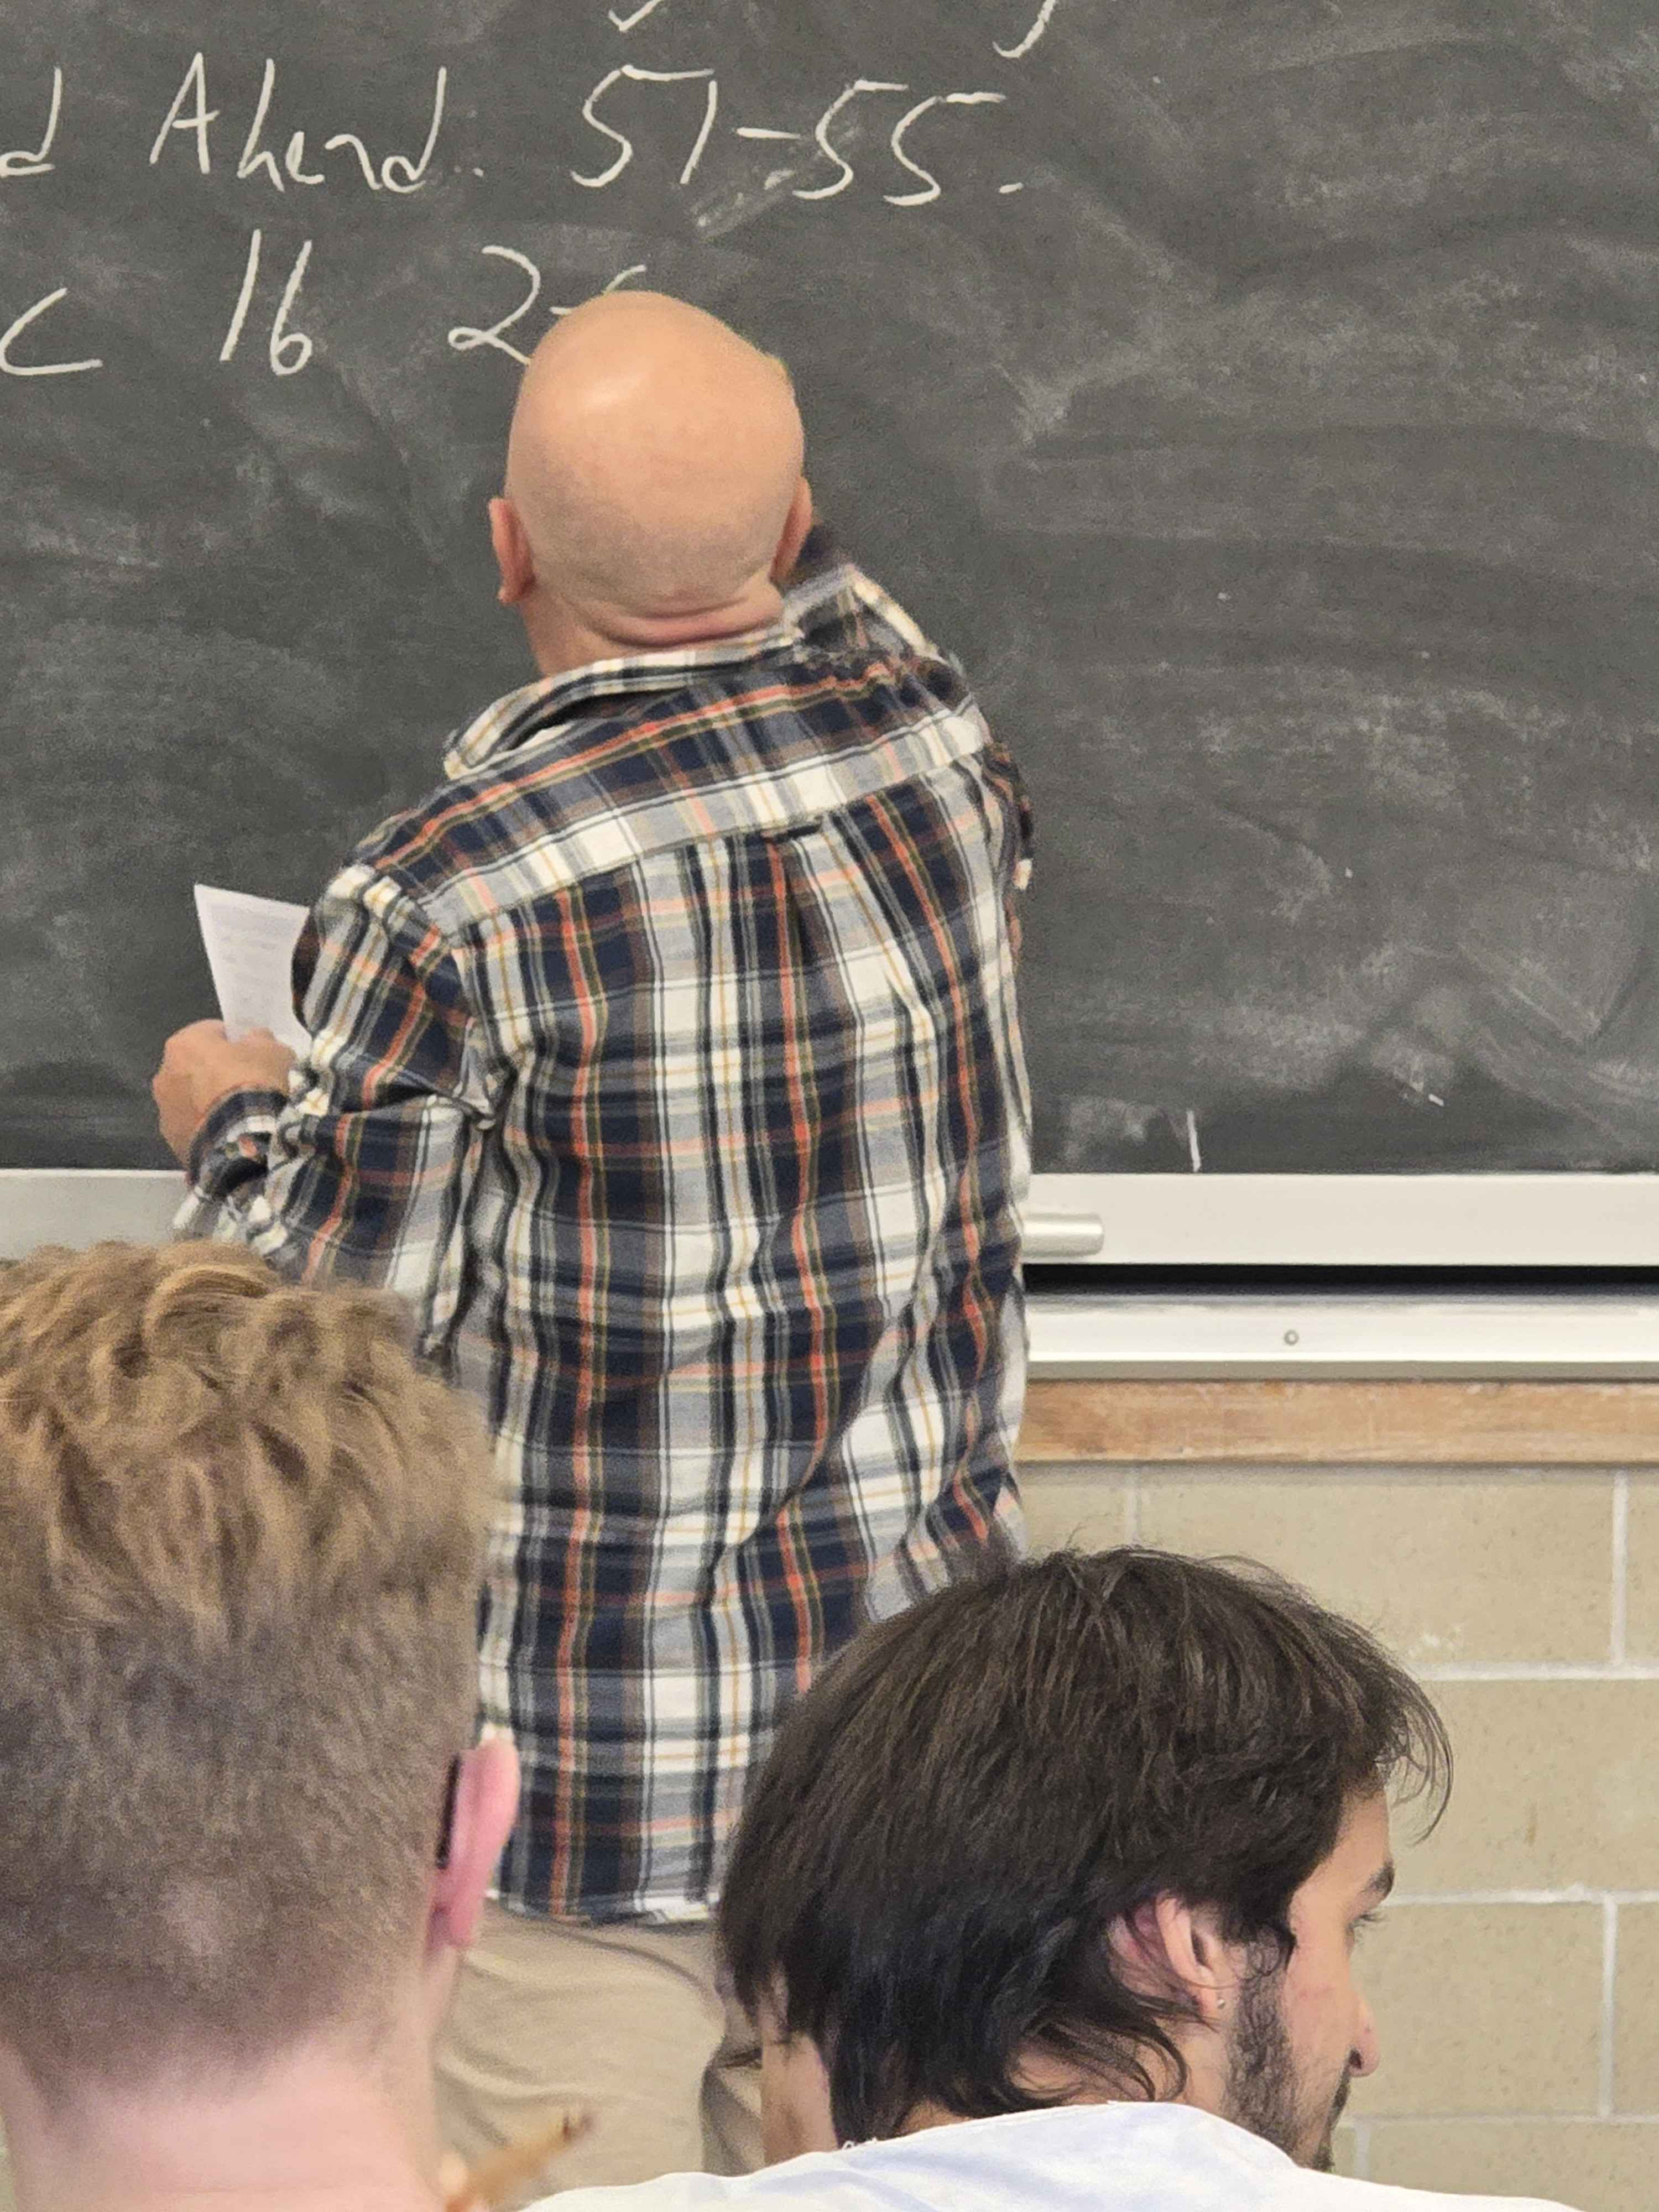
\includegraphics[scale=0.1]{MAT327 Notes/Dror Shirts/dror day 17 shirt.jpg}
\end{figure}

\noindent Turns out, we are bad at telling spaces apart (in terms of homeomorphisms). Here are some examples.
\begin{itemize}
    \item Closed intervals and open intervals are not homeomorphic because one is compact, and the other isn't.
    \item Open intervals and half-open intervals are not homeomorphic either, since if we remove a point in an open interval, it would cause a disconnection, while we may remove the point at the closed end of the half-open interval and retain connectedness.
    \item Consider $D_0, D_1, D_2, \dots$, i.e. $D_i$ is an open disc with $i$ disjoint open discs removed from it (read: punctured disc).
    \item Surfaces of different genus are not homeomorphic, but we don't have the tools to prove it yet.
    \item The circle and the trefoil knot are homeomorphic, since we may parameterize the curves (read: \href{https://en.wikipedia.org/wiki/Jordan_curve_theorem}{Jordan curve theorem}; simple closed curve is homeomorphic to $S^1$.)
\end{itemize}

\newpage
\noindent We start with some fundamental definitions in group theory.
\begin{definition}
    A group is a set $G$ along with the three following operations:
    \begin{itemize}
        \item $m : G \times G \to G$, i.e., multiplication. Note that in practice, we will never write $m$ as multiplication, we're just writing it as a function for now, where $(a, b) \mapsto m(a, b) = a \cdot b = ab$.
        \item $\iota : G \to G$, $a \mapsto \iota(a) = a^{-1}$, i.e. the unary operation, or the inverse.
        \item $e = 1 \in G$, called the nullary operation; it specifies ``the unit'' in the group $G$.
    \end{itemize}
\end{definition}
\noindent Groups satisfy the axioms,
\begin{enumerate}[label=(\alph*)]
    \item Associativity; for $a, b, c \in G$, we have $(ab)c = a(bc)$.
    \item Identity; for $a \in G$, $ea = ae = a$.
    \item Inverse; $a a^{-1} = a^{-1} a = 1 = e$.
\end{enumerate}
We now give some examples.
\begin{enumerate}[label=(\alph*)]
    \item If $V$ is a vector space, we have that it is also a group with $m = +$, $\iota = (v \mapsto -v)$, and $e = 0$, i.e. $1_G = 0_V$.
    \item The integers $\ZZ$ equipped with the addition operation is a group, i.e. $(\ZZ, +)$.
    \item The integres modulo $2$, $\ZZ/2\ZZ = \{0, 1\}$, equipped with multiplication is a group, i.e. $(\ZZ/2\ZZ, \times)$.
    \item The real numbers equipped with $+$ is a group, i.e. $(\RR, +)$.
    \item The real numbers without $\{0\}$ equipped with $\times$ is also a group, i.e. $(\RR \setminus \{0\}, \times)$.
    \item $(\RR_{>0}, \times)$ is a group.
    \item $(\QQ \setminus \{0\}, \times)$ and $(\CC \setminus \{0\}, \times)$ are also groups.
\end{enumerate}
It happens that each of these five examples are such that their elements commute under their respective operations. It is not required for elements to commute for them to form a group; when they do, we call them Abelian.
\begin{enumerate}[label=(\alph*)]
    \setcounter{enumi}{7}
    \item The set of all invertible $n \times n$ matrices with entries in $\CC$, equipped with multiplication, i.e. $\GL_n(\CC)$, is not commutative. Specifically, we have $m : (A, B) \mapsto AB$ (matrix multiplication), $e = I_n$, and $\iota$ being the matrix inversion operation.
\end{enumerate}
\begin{simpleclaim}
    In any group, $(ab)^{-1} = b^{-1}a^{-1}$.
\end{simpleclaim}
\noindent We simply have $(ab)(b^{-1}a^{-1}) = a e a^{-1} = a a^{-1} = e$. \qed
\begin{enumerate}[label=(\alph*)]
    \setcounter{enumi}{8}
    \item Let $[n] = \{1, \dots, n\}$. $S_n = \{\sigma : [n] \to [n] \mid \sigma \text{ is invertible } \iff \sigma \text{ inj. and cont.} \}$. Then the set of permutations forms a a group under function composition, i.e. $\KS_n = (S_n, \circ)$.
    \item Given any set $X$,
    \[ S(X) = \{\sigma : X \to X \mid \sigma \text{ is invertible } \} \]
    is a group under function composition, $(S(X), \circ)$.
    \item \textit{Relations of a cube:} There are $24$ different rotations of a cube; let these moves be given by $S_C$. We note that these moves are non-commutative under composition (i.e., swapping the order of moves).
    \item Let $G$ be the set of possible combinations we can get on a Rubik's cube with legal moves. Then we have
    \[ \abs{G} = \frac{8! \cdot 3^8 \cdot 12! \cdot 2^12}{12} = 43,252,003,274,489,856,000. \]
\end{enumerate}
\begin{definition}
    If $G_1, G_2$ are groups, then a homomorphism $\varphi : G_1 \to G_2$ is a function such that $\varphi(ab) = \varphi(a) \varphi(b)$, $\varphi(a^{-1} = \varphi(a)^{-1}$, and $\varphi(e_{G_1}) = e_{G_2}$.
\end{definition}
We now give some examples of group homomorphisms.
\begin{enumerate}[label=(\alph*)]
    \item The inclusion map yields the following embeddings,
    \[ (\ZZ, +) \hookrightarrow{} (\QQ, +) \hookrightarrow{} (\RR, +) \hookrightarrow{} (\CC, +). \]
    \item $\pi : \ZZ \to \ZZ/2\ZZ = \{0, 1\}$ is another example of a morphism, where $\pi(k) = 0$ if $k$ is even, and $1$ if $k$ is odd. 
    \item $\det : \GL_n(\CC) \to (\CC \setminus \{0\}, \times)$, where $\det (AB) = \det (A) \det B)$. 
    \item $\alpha : \KS_n \to \KS_{n+1}$, where $\alpha$ is sort of an ``inclusion'' map in the sense that we permute the first $n$ elements as $\sigma \in S_n$ does, and we fix the $n+1$th element to yield a permutation in $S_{n+1}$.
    \item $\beta : \KS_4 \to \KS_3$. $S_4$ is the set of rotations of a tetrahedron. Permutations $\sigma \in S_4$ permute the positions of the vertices; then we may partition the edges of the tetrahedron (of which there are $6$) into $3$ pairs of non-adjacent sides; since there are only $3$ possible positions for the pairs of edges to go to, we see $\sigma \in S_4$ induces a permutation of pairs of edges, i.e. on $S_3$ (reference: \href{https://math.stackexchange.com/questions/3365927/homomorphism-from-s-4-to-s-3}{here}). We can check that this is a homomorphism because it preserves multiplicative structure.
\end{enumerate}

\noindent We now move back to fundamental groups. There was some discussion in class on why the $1$-torus and $2$-torus are not homeomorphic by the fundamental group, but I don't really understand it.
\begin{definition}
    A path in a topological space $X$ is a continuous function $\gamma : [0, 1] \to X$.
\end{definition}
\begin{definition}
    Paths $\gamma_0, \gamma_1 \in X$ are called \textit{path-homotopic} if $\gamma_0 \sim_p \gamma_1$, i.e. there exists a continuous function $H = H(s, t) : [0, 1]_s \times [0, 1]_t \to X$ such that for all $s, t \in [0, 1]$, $H(s, 0) = \gamma_0(s)$, $H(s, 1) = \gamma_1(s)$, $H(0, t) = \gamma_0(0) = \gamma_1(0)$, and $H(1, t) = \gamma_0(1) = \gamma_1(1)$.
\end{definition}
\noindent Intuitively, the idea is that we can deform $\gamma_0$ to $\gamma_1$ while fixing the endpoints. Think of $s$ as the ``where you are on the curve'' parameter and $t$ as the time parameter.
\begin{simpleclaim}
    $\sim_p$ is an equivalence relation.
\end{simpleclaim}
\noindent We check $\sim_p$ satisfies reflexivity, symmetry, and transitivity below respectively.
\begin{enumerate}[label=(\alph*)]
    \item By the homotopy, we have $\gamma \sim_p \gamma$, i.e. $H(s, t) = \gamma(s)$.
    \item Suppose $\gamma_0$ is path-homotopic to $\gamma_1$. This means there exists $H$ s.t. $H(s, 0) = \gamma_0(s)$ and $H(s, 1) = \gamma_1(s)$. Define $H'(s, t) = H(s, 1-t)$; then
    \begin{align*}
        H'(s, 0) &= H(s, t) = \gamma_1(s), \\
        H'(s, 1) &= H(s, 0) = \gamma_0(s).
    \end{align*}
    So $\gamma_1 \sim_p \gamma_0$.
    \item Let $\gamma_0 \sim_p \gamma_1$ by $H'$, and $\gamma_1 \sim_p \gamma_2$ by $H''$. Define
    \[ H(s, t) = \begin{cases} H'(s, 2t) & t \leq \frac{1}{2}, \\ H''(s, 2t - 1) & t \geq \frac{1}{2}. \end{cases} \]
    This gives $\gamma_0 \sim_p \gamma_2$ by $H$.
\end{enumerate}
We give some examples. In $\RR^n$, if $\gamma_0(0) = \gamma_1(0)$ and $\gamma_0(1) = \gamma_1(1)$, then $\gamma_0 \sim_p \gamma_1$, since we may construct
\[ H(s, t) = (1 - t) \gamma_0(s) + t \gamma_1(s). \]
 